\documentclass[a4paper,11pt ]{xc_webpage_project}
\usepackage[utf8]{inputenc}
\usepackage[spanish,english]{babel}
\usepackage{graphicx}
\usepackage[labelsep=period]{caption}
\usepackage{parallel}
\usepackage{wrapfig} %% Wrapping text around figures.
\usepackage{caption}
\usepackage{subcaption}

\renewcommand{\titProject}{Pasarela sobre la línea de cercanías C-5 en Alcorcón}
\def\@anagramFont{\relax}
\renewcommand{\client}{Ayto. de Alcorcón}
\renewcommand{\dateProject}{2022}
\renewcommand{\location}{Alcorcón (España)}
\renewcommand{\widhtLeftCol}{0.475\textwidth} % normalmente no lo cambiaremos
\renewcommand{\widhtRightCol}{0.475\textwidth} % normalmente no lo cambiaremos


\begin{document}
\headerSpanish

\begin{Parallel}{\widhtLeftCol}{\widhtRightCol}
  \ParallelLText{
    El paso de peatones y ciclistas sobre la línea del tren de cercanías a la altura de la calle Argentina, se realiza a través de sendas aceras de dimensiones muy reducidas. Por este motivo, el Ayuntamiento de Alcorcón decidió abordar la ampliación del paso superior existente con el proyecto de una pasarela de 8 m ancho que soportara el intenso tráfico de peatones y ciclistas de forma cómoda y segura. La actuación se completa con la ejecución de una vía ciclista para conectar la pasarela con los itinerarios existentes, así como la ampliación de aceras y zonas peatonales para dotar de accesibilidad al entorno.

    Los condicionantes de diseño de la pasarela vinieron muy determinados por la presencia de la línea férrea: reducir al mínimo posible las operaciones que afecten a la vía,  control de riesgos durante la construcción, minimizar al máximo las necesidades de mantenimiento (ausencia de apoyos elastoméricos,\ldots); en resumen, plantear una estructura duradera, monolítica y racional.
  }
  
  \ParallelRText{
    The passage of pedestrians and cyclists over the suburban train line at Argentina Street is carried out through very narrow sidewalks. For this reason, the Alcorcón City Council decided to address the expansion of the existing overpass with the project of an 8 m wide walkway that would withstand the heavy traffic of pedestrians and cyclists comfortably and safely. The action is completed with the execution of a cycle path to connect the footbridge with the existing routes, as well as the widening of sidewalks and pedestrian areas to provide accessibility to the neighboring areas.

     The footbridge design constraints were highly determined by the presence of the railway line: reduce to the minimum possible those operations that affect the tracks, risk control during construction, minimize maintenance needs as much as possible (absence of elastomeric supports, \ldots); in short, propose a lasting, monolithic and rational structure.
}

\end{Parallel}
\begin{figure}[h]
\centering
\begin{subfigure}{\widhtLeftCol}
  \includegraphics[width=\textwidth]{figures/acera_estrecha}
  \caption{Estrangulamiento de acera en calle Argentina.}
\end{subfigure}
 \hfill
\begin{subfigure}{\widhtRightCol}
    \includegraphics[width=\textwidth]{figures/tablero_NE.jpg}
    \caption{Paso superior al que se adosa la pasarela.}
\end{subfigure}
\end{figure}

\begin{Parallel}{\widhtLeftCol}{\widhtRightCol}
  \ParallelLText{Se diseña una pasarela integral, de un solo vano con 20 m de luz. El tablero está constituido por una estructura nervada pretensada, prefabricada en módulos que se colocan adyacentes uno a otro, evitando de este modo la necesidad de instalar prelosas. Debido a las limitaciones del espacio de trabajo y con el fin interferir lo menos posible con los usuarios de las vías y espacio público y con el propio espacio ferroviario, la cimentación es profunda con 8 micropilotes de 177,8 mm de diámetro en cada estribo. Sobre el encepado se hormigona la viga riostra que conecta los nervios de la losa prefabricada. 
}
  \ParallelRText{An integral footbridge is designed, with a 20  m single span. The deck is made up of a prestressed ribbed structure, prefabricated in modules that are placed adjacent to each other, thus avoiding the need to install pre-slabs. Due to the limitations of the work space and in order to interfere as little as possible with the users of the train and public space and with the railway space itself, a deep foundation is designed with 8 micropiles in each abutment,  177.8 mm in diameter. The bracing beam that connects the nerves of the precast slab is concreted over the pile cap.

  }
\end{Parallel}

 \begin{figure}[h]
\centering
\begin{subfigure}{\widhtLeftCol}
  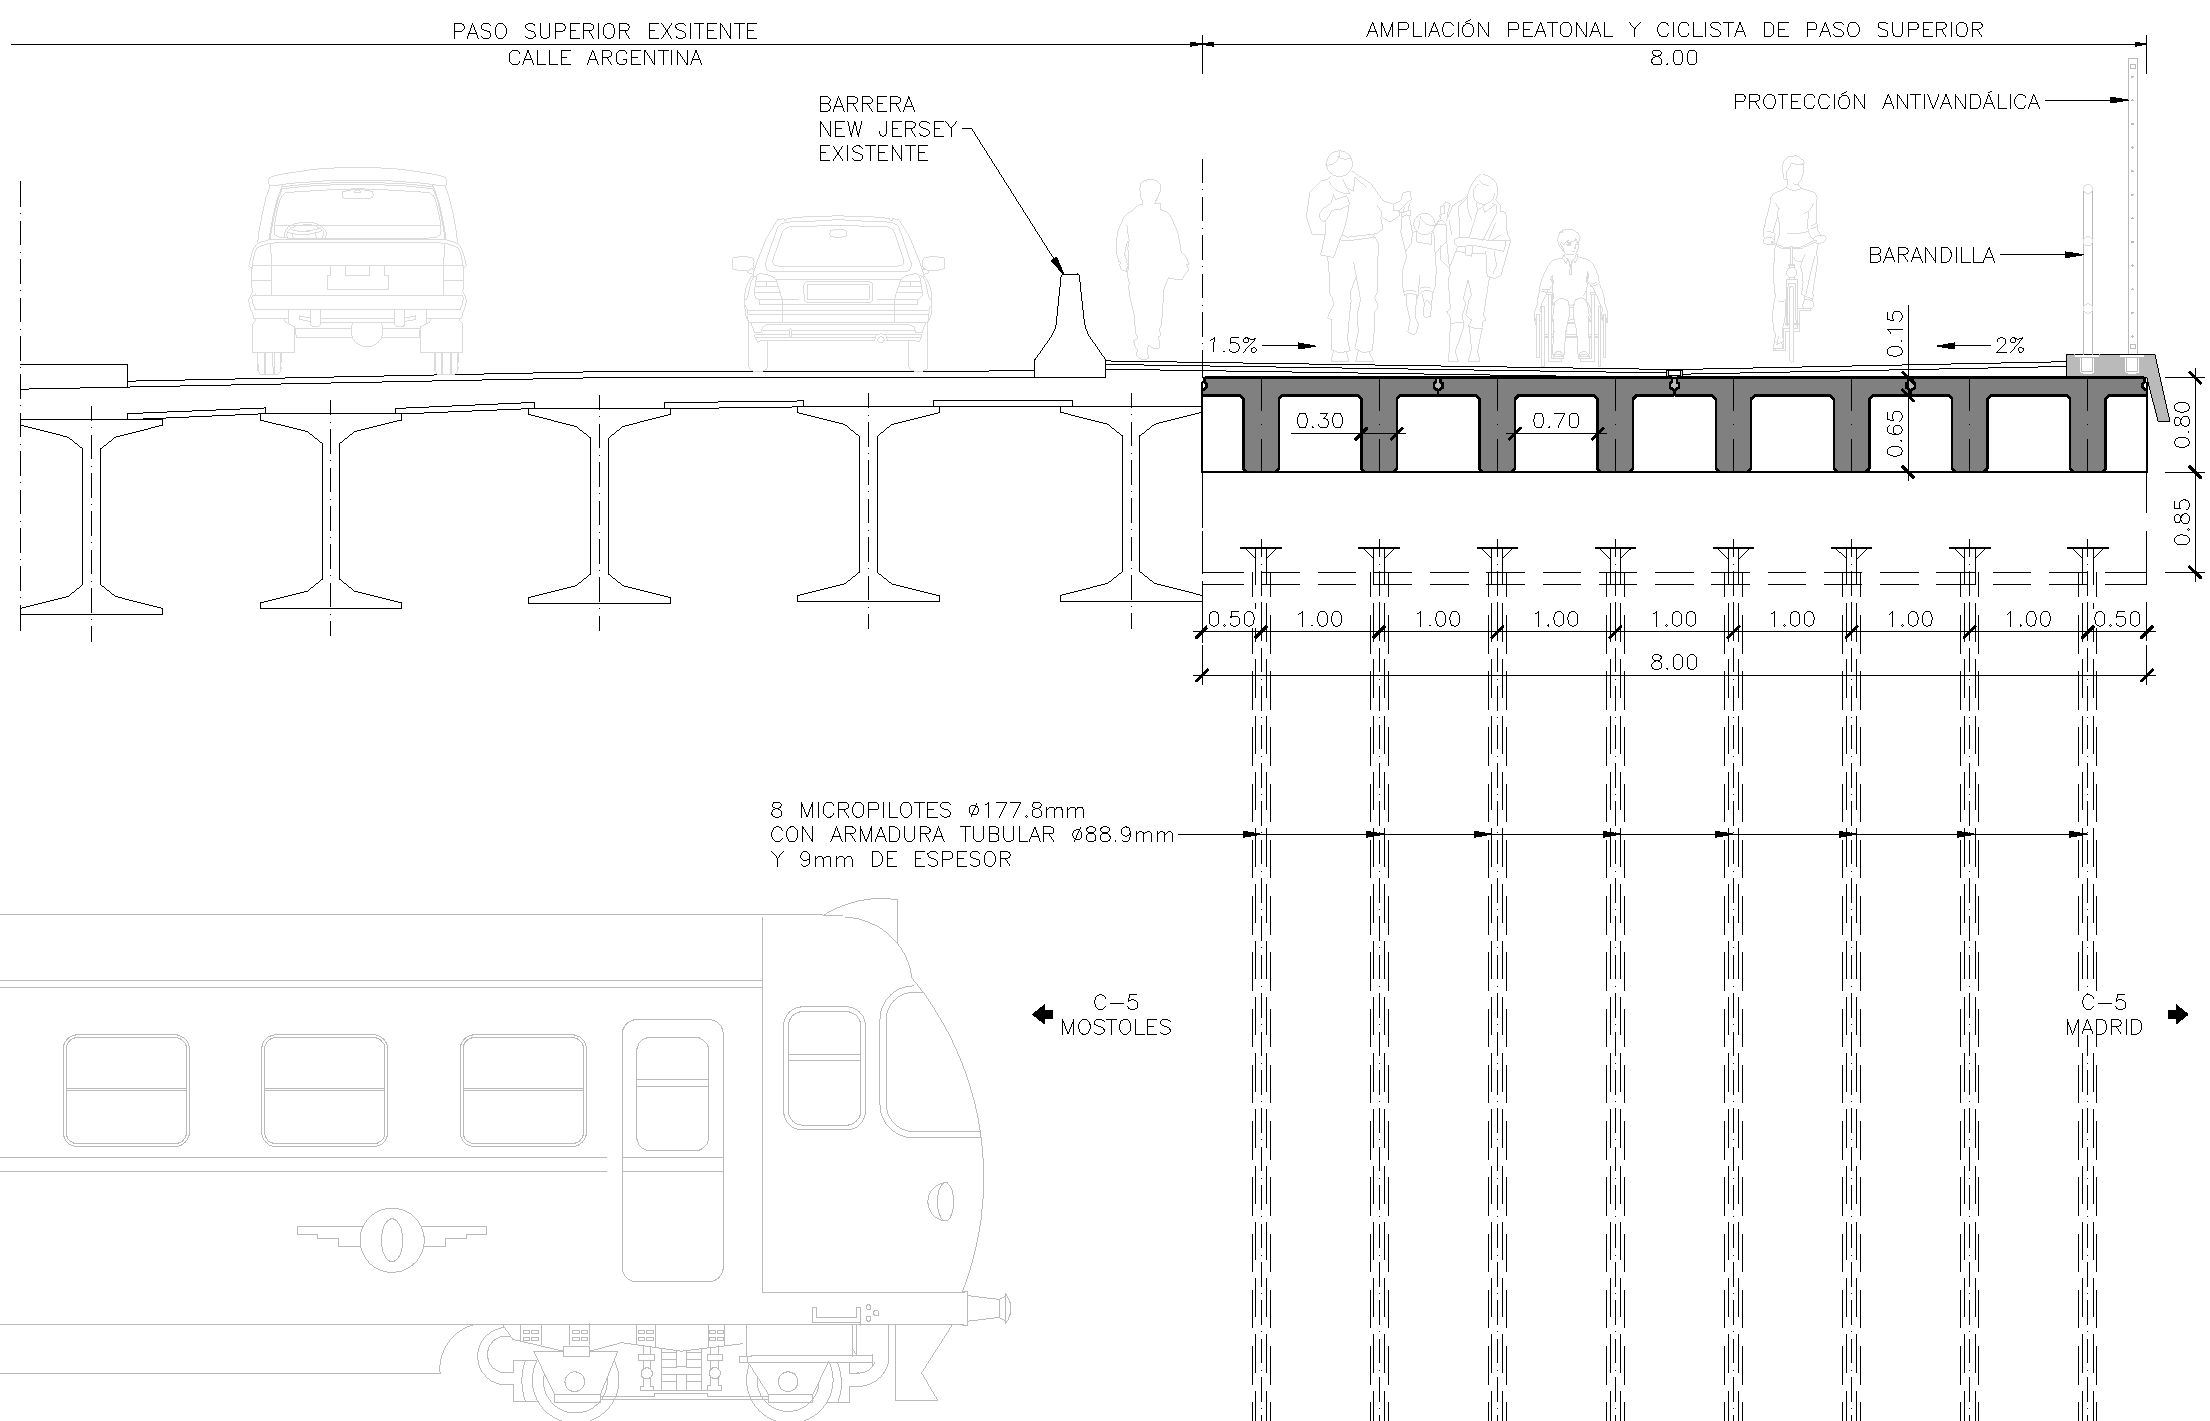
\includegraphics[width=\textwidth]{figures/sectrans_pasarela}
  \caption{Sección transversal de la estructura de la pasarela}
\end{subfigure}
 \hfill
\begin{subfigure}{\widhtRightCol}
    \includegraphics[width=\textwidth]{figures/perfil_pasarela}
    \caption{Perfil de la pasarela}
\end{subfigure}
\end{figure}
 
\begin{Parallel}{\widhtLeftCol}{\widhtRightCol}
  \ParallelLText{Sobre la pasarela proyectada se reserva un carril de 2,60 m bidireccional, para uso exclusivo de ciclistas, el cual se conecta con los itinerarios ciclistas existentes a uno y otro lado de la pasarela con el trazado de una vía ciclista. La obra se completa con varias actuaciones urbanísticas y de restauración paisajística en el entorno.
  }
  \ParallelRText{A 2.60 m bidirectional lane is reserved in the footbridge for the exclusive use of cyclists; the connection with the existing cycling routes on both sides of the footbridge is made by drawing a cycle path. The work is completed with various urban and landscape restoration actions in the surroundings.
  }
\end{Parallel}

\begin{figure}[h]
  \centering
  \includegraphics[width=120mm]{./Alcorcon_footbridge.png}
\end{figure}


\end{document}
  
